\documentclass[a4paper]{article}
\usepackage{amsmath} % for multi-line aligned equations
\usepackage{enumitem} % for bullet points
\usepackage{graphicx} % for displaying images
\graphicspath{ {./Images/} } % search path for images
\usepackage{booktabs} % for making tables in professional style with top and bottom border
\usepackage{textcomp} % for degree symbol
\usepackage{fullpage} % for reducing page margins
\usepackage{float}    % to keep figures with text

%opening
\title{Libration Point Orbit Rendezvous Technique Using Linearized Relative Motion Dynamics and Nonlinear Differential Correction}
\author{Sara Case\\ Department of Aerospace Engineering\\ University of Maryland, College Park}
\date{Spring 2015}

\begin{document}

\maketitle


\section{Short Abstract}

\newpage

\section{Extended Abstract}

So far, all libration point missions have consisted of a single satellite which operates independently of any other satellite.  There is research on deploying a formation of satellites to fly together around libration points.  However, not much research has been performed regarding rendezvous with libration point orbiters.

Libration point orbit rendezvous would be a critical component for many possible mission architectures.  If a large satellite needs to be launched in components and assembled in orbit, the individual components would need to perform rendezvous and docking prior to assembly.  If a valuable space asset such as a telescope requires an on-orbit repair, the satellite servicing mission will need to rendezvous with the object.  A libration point orbit could be a useful place to build a space station, and in that case rendezvous capabilities would be important during the construction of the station as well as every crew and cargo mission to visit the station.

Satellite rendezvous in low-Earth orbit is well-studied, due to many years of experience operating the International Space Station and other applications.  The Hill's / Clohessy-Wiltshire equations can be used to estimate the relative motion of a chaser vehicle with respect to a target vehicle in a circular orbit.  These equations of relative motion can be used to compute the estimated \(\Delta V\) (instantaneous change in velocity) to travel between waypoints defining an approach trajectory.  However, for libration point orbits, the dynamical environment is quite different and the same equations of motion can not be used.

Luquette \cite{luquette2004} has developed linearized equations of relative motion for formation flying in libration point orbits.  Lian et al. \cite{lian2011} have used these linearized dynamics to compute impulses for a chaser satellite to travel between waypoints in order to approach a target orbiting a libration point.  This paper discusses the results of applying this technique for test cases in the Earth-Moon L1 system, and presents an additional step in which the shooting method is used to refine the computed \(\Delta V\) for use in nonlinear propagation.

This paper presents an overview of the dynamics of the circular restricted three body problem (CRTBP), as well as the linearized equations of relative motion of a chaser satellite with respect to a target satellite orbiting in the restricted three body problem (RTBP) derived by Luquette \cite{luquette2004}. These equations of motion are valid anywhere in the RTBP system; they are not assumed to be near any specific libration point. They can also be used for any type of libration point orbit, including halo and Lissajous orbits. These equations are functions of the offset state of the chaser vehicle with respect to the target vehicle in the rotating frame; the position of the target vehicle in the rotating frame with respect to the origin; the mass ratio of the primary bodies, and the rotation rate of the rotating frame.

In order to integrate a chaser satellite's trajectory using these equations of relative motion, the integration state vector must contain the absolute state of the target satellite in the CRTBP frame (with respect to the origin of the CRTBP frame) and the relative state of the chaser satellite in the CRTBP frame (with the origin located at the target satellite).  The target satellite's state over time can be integrated using the classical CRTBP equations of motion, which must be done concurrently with the integration of the relative motion of the chaser so that the time-dependent linearized relative motion dynamics matrix can be computed.

The concept of waypoints can be used to divide a rendezvous approach trajectory into a series of shorter segments.  The starting and ending waypoints of a segment are defined with respect to the location of a target satellite.  When considering rendezvous with a satellite in a circular orbit, the Clohessy-Wiltshire or Hill's equations can be used as a linearized dynamics model for a chaser satellite with respect to a target satellite.  The inverse of the linear dynamics matrix is used to compute the velocity required to travel from one waypoint to the next within a specified amount of time.  This approach can also be applied in the RTBP using the linear dynamics matrix derived by Luquette.  The procedure for this is presented in the paper.

In  \cite{lian2011}, Lian et. al. used this approach using the RTBP relative motion dynamics derived by Luquette. 

The approach described above for computing \(\Delta V\) is based on the linearized equations of relative motion developed by Luquette.  Of course, the true dynamical environment in the CRTBP is nonlinear. The linear-based estimate of \(\Delta V\) can be ``corrected" for the nonlinear propagation model using the shooting method of differential correction.  The linear-based estimated velocity is used as an initial guess for the iterative process.  Each of the three components of the velocity vector is varied in order to achieve convergence on the desired three-dimensional waypoint within some specified tolerance. This differential correction procedure is presented in the paper.

Also discussed are the definitions of local RIC (radial-intrack-crosstrack) and VNB (velocity-normal-binormal) reference frames, defined with respect to the target satellite's orbit around its libration point.  Each of these frames will rotate once for each full orbit of the target around the libration point, with the origin of both frames located at the target satellite's position. 

The performance of these techniques are evaluated with various test cases. Figure \ref{fig:RIC_1} 

The target satellite is in a planar Lyapunov orbit around the Earth-Moon L1 point. For this test, the rendezvous starts with the target satellite on the CRTBP +X-axis, that is, crossing the XZ-plane.

Three waypoints are defined for the chaser satellite to travel along on its rendezvous with the target, with a final waypoint located at the target satellite itself.  Note that these waypoints represent an approach along the \(\mathbf{I}\) axis of the RIC frame. 

Figure \ref{fig:RIC_1} shows the result of propagating the target and chaser satellite through a rendezvous using these waypoints.  The integration is performed in the CRTBP frame, and the results are converted to the RIC frame for visualization, with the target spacecraft at the origin and the chaser spacecraft offset with respect to the target shown in kilometers.  The green curve shows the path of the chaser satellite when propagated using the linear relative motion dynamics, with the application of impulsive \(\Delta V\)'s as computed using the \textbf{linearized dynamics matrix.}  The model used to compute the impulsive maneuvers matches the linear propagation model, and so the chaser satellite travels precisely to each waypoint.  The red curve shows the result when the chaser satellite is propagated using the nonlinear CRTBP dynamics when the nominal \(\Delta V\)'s as computed using the linear model are still applied.  It is easily seen that the nominally planned maneuvers do not bring the chaser exactly to the desired waypoints when propagating with the nonlinear model.  Finally, the blue curve shows the result when the chaser satellite is propagated using the nonlinear CRTBP dynamics and the \(\Delta V\)'s have been corrected through the iterative shooting method procedure.  The path does not precisely match the original green curve due to the different dynamical models in use; however, each waypoint is achieved successfully.  % TODO: (Also note that the image axes are not scaled equally.)

\begin{figure}[h] 
	\begin{center}
		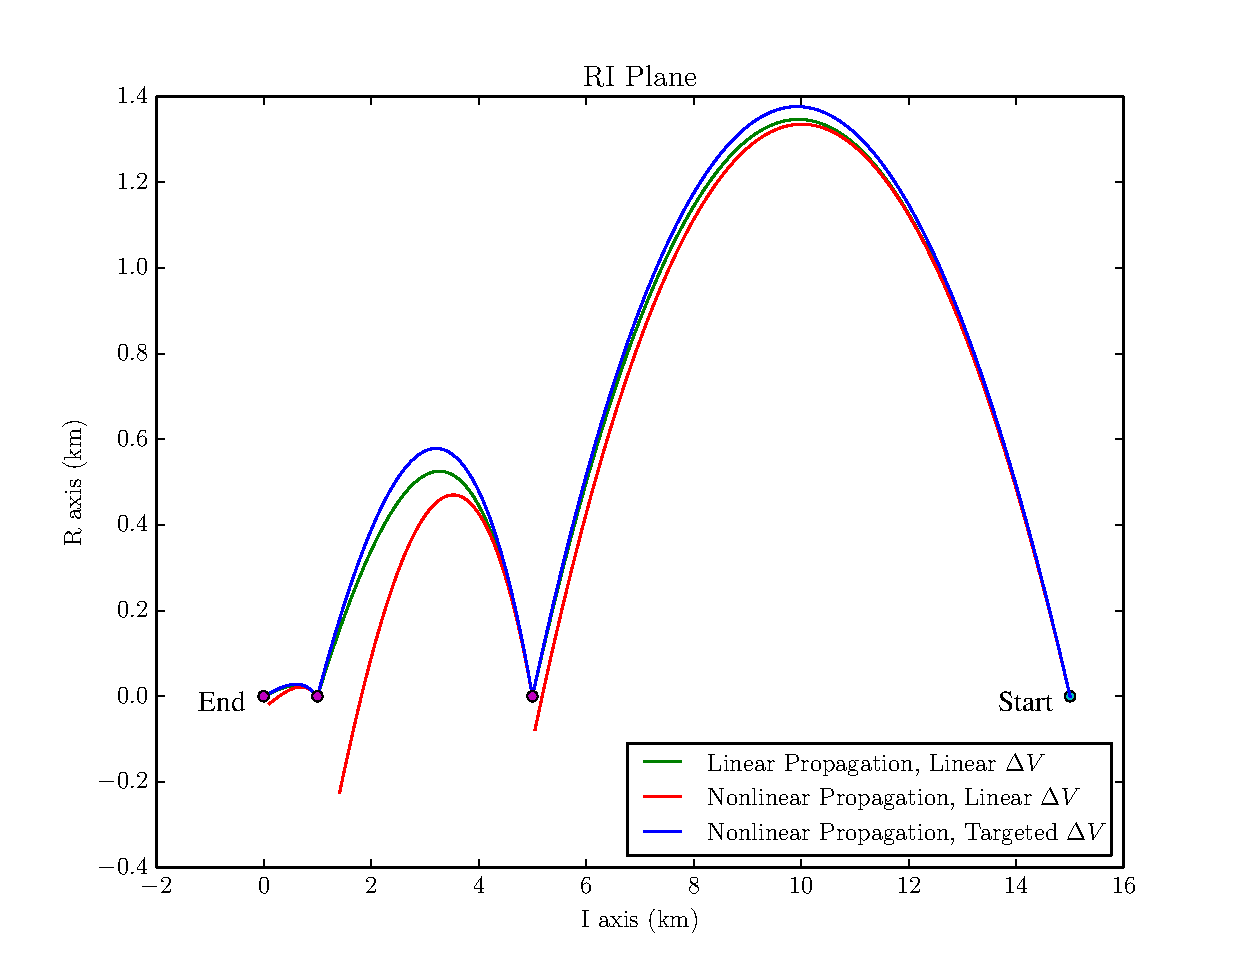
\includegraphics[width=0.9\textwidth]{RIC_1}
		\caption{Relative Motion of a Chaser Satellite with respect to a Target (km)}
		\label{fig:RIC_1}
	\end{center}
\end{figure} % TODO: add more context/description to the captions for the plots

The magnitude of the differences in \(\Delta V\) are compared between the linear computation and the targeted computation, as well as the angular difference between the two \(\Delta V\) vectors, and the resulting differences in achieved position errors.

This technique can be used to evaluate the relative \(\Delta V\) cost of performing a rendezvous at different starting points along the target spacecraft's orbit.  Due to the differing local curvature of the target orbit at different starting locations, the relative motion patterns in the RIC frame for each rendezvous are different. Also discussed are the relative costs of approaching the target satellite, for example, rendezvous approach sequences along the primary axes of the RIC frame.

\clearpage

\bibliographystyle{unsrt}
\bibliography{LPORendezvous}

\end{document}
